%%%% Document type  %%%%
\documentclass[preprint,12pt,fleqn]{article}
 \usepackage{ragged2e}
\usepackage{authblk}  % Package for author affiliations
% \usepackage{nopageno} % no page numbers
\usepackage{placeins} % \FloatBarrier

\usepackage[most]{tcolorbox}
\newtcolorbox[auto counter,number within=chapter]{definition}[1][]{
  enhanced,
  breakable,
  fonttitle=\scshape,
  title={Definition \thetcbcounter},
  #1
}

%%%% Document structure %%%%
%\usepackage{geometry}
\usepackage[verbose=true,letterpaper]{geometry}
\geometry{
%    a4paper,
%    left=30mm,
%    right=30mm,
%    top=30mm,
%    bottom=30mm,
    textheight=9in,
    textwidth=6in,
    top=1in,
    headheight=12pt,
    headsep=25pt,
    footskip=30pt,
   % phone  
   %a5paper,
   %width=120mm,
  %height=180mm,
}

\usepackage{lineno} % used along with \linenumbers after begin document. 
\usepackage{setspace} 
% \setstretch{1.4}
\makeatletter % The following lines get rid of footer stating pre-preint to elsevier.
\def\ps@pprintTitle{%
\let\@oddhead\@empty
\let\@evenhead\@empty
\def\@oddfoot{}%
\let\@evenfoot\@oddfoot}
\makeatother
\graphicspath{ {../images/} }
\usepackage{pgf} % calculate cohort stats percentage

%%%% Bibliography   %%%%
\usepackage{natbib}
\setcitestyle{numbers,sort&compress}
\setcitestyle{sort&compress}
\usepackage{hypernat} 
    
%%%% Aesthetics     %%%%
\usepackage{microtype}
% \RequirePackage{times} % Font
\usepackage{ccaption}
\usepackage{siunitx}
\usepackage[T1]{fontenc}
\usepackage[utf8]{inputenc}
\usepackage{nameref}% this allows a reference be named, to print unnumbered references by their section name (used here for linking to Supplemental text in this case).

%%%% Paragraph Formatting %%%
\setlength{\parindent}{0pt}
\setlength{\parskip}{6pt plus 2pt minus 1pt}

%%%% Supplemental labels%%%%
%Define command to start a supplemental section
%set the supplemental letter used for figures (e.g. Figure E1)
\newcommand{\beginsupplement}{%
        \setcounter{table}{0}
        \renewcommand{\thetable}{S\arabic{table}}%
        \setcounter{figure}{0}
        \renewcommand{\thefigure}{S\arabic{figure}}%
         }

%%%% Building tables%%%%
\usepackage{booktabs} % required for tables
\usepackage{rotating,tabularx} 
\newcolumntype{Z}{ >{\centering\arraybackslash}X } % defining table content layout per box
\usepackage{ltablex} % allow page break between lines in tabularx
% \usepackage{caption} \captionsetup{font=normalsize} % to set the caption size as normal even when table is tiny.
\usepackage{multirow}
\usepackage{pdflscape}

%%%% Colors %%%%
\usepackage{xcolor} 
\definecolor{natureblue}{RGB}{5,110,210}
    \usepackage[colorlinks]{hyperref} 
\AtBeginDocument{%this allows colours to chage from the defined elsearticle template.
\hypersetup{
    	colorlinks=true,
        linkcolor={natureblue},
    	citecolor={natureblue},
        filecolor=blue!50!black,
        urlcolor=cyan,
    	}}

\definecolor{kispiblack}{HTML}{333333}
\definecolor{kispidarkblue}{HTML}{023047}
\definecolor{kispidarkgreen}{HTML}{006666}
\definecolor{kispired}{HTML}{C70000}
\definecolor{kispilink}{HTML}{007DB8}%219EBC
% \color{kispi_black} %default
\definecolor{kispiblue}{HTML}{701A57}
% City sunset: https://www.color-hex.com/color-palette/40131
\definecolor{colorSUNSET1}{HTML}{eeaf61}
\definecolor{colorSUNSET2}{HTML}{fb9062}
\definecolor{colorSUNSET3}{HTML}{ee5d6c}
\definecolor{colorSUNSET4}{HTML}{ce4993}
\definecolor{colorSUNSET5}{HTML}{6a0d83}
\definecolor{natureblue}{RGB}{5,110,210}    
\usepackage{dirtree}  % Load the dirtree package


% command to use these colors and formatting; xspace for correct spacing including with punctuation marks.
\usepackage{xspace}
\newcommand{\variablesdarkgreen}[1]{\textbf{\textcolor{kispidarkgreen}{#1}}\xspace}

%%%% Fancy stuff %%%%
%\usepackage{fancyhdr}
%\pagestyle{fancy}
%\lhead{My Name}
%\chead{}
%\rhead{\thepage}
%\cfoot{} % get rid of the page number 
%\renewcommand{\headrulewidth}{0pt}
%\renewcommand{\footrulewidth}{0pt}
 
 
%\usepackage{fancyhdr}
%\usepackage{lastpage}
%\pagestyle{fancy}
%\fancyhf{}
%\rfoot{\thepage}
%\cfoot{} % get rid of the page number 
%\renewcommand{\headrulewidth}{0pt}
%\renewcommand{\footrulewidth}{0pt}

 
\usepackage{tocloft}  % Customizing the Table of Contents
\setcounter{tocdepth}{2}


%%%% Include code %%%%
% \usepackage{verbatim}

\usepackage{listings}
\lstset{
    basicstyle=\ttfamily\small,
    breaklines=true,
    postbreak=\mbox{\textcolor{red}{$\hookrightarrow$}\space}, % 
    breakatwhitespace=false,
    % frame=single,
    showstringspaces=TRUE, % Don't show spaces in strings as special characters
    tabsize=2, 
    language=sh 
}

\usepackage{fontspec}
% \setmainfont{IBM Plex Sans}
% \setmonofont{IBM Plex Mono}
% \usepackage{unicode-math}
% \setmathfont{IBM Plex Math}

%\renewcommand{\rmdefault}{ptm}
%\renewcommand{\sfdefault}{phv}


% {{\ttfamily \hyphenchar\the\font=`\-} % set hyphenation for texttt blocks









% nips 2017 settings


\usepackage[printonlyused,withpage,nohyperlinks]{acronym}

\begin{document}
\title{PanelAppRex aggregates disease gene panels and facilitates sophisticated search}	

% in your preamble, before \author:
\newcommand{\QUANT}{1}
\newcommand{\GHI}{2}
\newcommand{\LEEDS}{3}
\newcommand{\IPSNEO}{4}
%\newcommand{\KISPIIMM}{3}
% \newcommand{\METAB}{4}

\author[\QUANT]{Quant Group} 
\author[\GHI]{Simon Boutry}% \textsuperscript{†}}
\author[\GHI]{Ali Saadat}% \textsuperscript{†}} \textsuperscript{†}}
%\author[\METAB]{D. Sean Froese}
\author[\LEEDS]{Sinisa Savic}% orcid.org/0000-0001-7910-0554
\author[\IPSNEO]{Luregn J. Schlapbach}
\author[\GHI]{Jacques Fellay}
\author[\IPSNEO]{Dylan Lawless \thanks{Addresses for correspondence: \href{mailto:Dylan.Lawless@kispi.uzh.ch}{Dylan.Lawless@kispi.uzh.ch}}
}

%\author[\KISPIIMM]{Maarja Soomann}% \textsuperscript{†}} \textsuperscript{†}}
%\author[\KISPIIMM]{Johannes Trück}
\affil[\QUANT]{The quantitative omic epidemiology group.} 
\affil[\GHI]{Global Health Institute, School of Life Sciences, École Polytechnique Fédérale de Lausanne, Switzerland.}
\affil[\LEEDS]{Leeds Institute of Rheumatic and Musculoskeletal Medicine, University of Leeds, Leeds, UK.}
\affil[\IPSNEO]{Department of Intensive Care and Neonatology, University Children's Hospital Zurich, University of Zurich, Zurich, Switzerland.}

% \affil[\METAB]{Division of Metabolism and Children’s Research Center, University Children’s Hospital Zürich, University of Zurich, Zurich, Switzerland.}



%\affil[\KISPIIMM]{Division of Immunology and the Children’s Research Center, University Children’s Hospital Zurich, University of Zurich, Zurich, Switzerland.}

\maketitle
\justify

%  Word count: ~2560

\clearpage
\begin{abstract}
\noindent \textbf{Purpose:}\\
Gene panel data are essential for variant interpretation and genomic diagnostics, but existing resources are fragmented, inconsistently annotated, and not easily accessible for programmatic use. 

\vspace{1em}
\noindent \textbf{Methods:}\\
We developed PanelAppRex, a harmonised dataset and interactive search tool that integrates over 58,000 curated gene-disease panel associations, including NHS-approved diagnostic panels. It supports natural language-style queries by gene, phenotype, disease group, and mode of inheritance (MOI), with results returned in machine-readable export formats. 

\vspace{1em}
\noindent \textbf{Results:}\\
In benchmarked case studies of immune disease diagnostics, the system achieved 100\% accuracy in identifying the most relevant gene panel. The underlying dataset includes standardised gene identifiers, disease annotations, MOI, and literature support, enabling seamless integration into bioinformatic pipelines. 

\vspace{1em}
\noindent \textbf{Conclusion:}\\
PanelAppRex aids genetic diagnosis and establishes a structured foundation for modelling genome-wide diagnostic priors for supporting evidence-aware variant interpretation.

\vspace{1em}
\noindent \textbf{Availability:} The platform data is openly available at  PanelAppRex base [Data set], Zenodo \url{https://doi.org/10.5281/zenodo.15736689}, with
source code at \url{https://github.com/DylanLawless/PanelAppRex},
and demonstration page at \url{https://DylanLawless.github.io/panelapprex.github.io/landing_page.html}. 
PanelAppRex is available under the MIT licence. 
The dataset is maintained for a minimum of two years following publication.
\end{abstract}
\clearpage

\section*{Acronyms}
\renewenvironment{description} % Internally acronym uses description which we redefine to make condense spacing. 
{\list{}{\labelwidth0pt\itemindent-\leftmargin
    \parsep-1em\itemsep0pt\let\makelabel\descriptionlabel}}
               {\endlist}
\begin{acronym} 
\acro{ad}[AD]{Autosomal dominant}
\acro{ar}[AR]{Autosomal recessive}
\acro{api}[API]{Application Programming Interface}
\acro{csv}[CSV]{comma-separated values}
\acro{ge}[GE]{Genomics England}
\acro{hgnc}[HGNC]{Human genome organisation Gene Nomenclature Committee}
\acro{iei}[IEI]{Inborn Errors of Immunity}
\acro{iem}[IEM]{Inborn Errors of Metabolism}
\acro{html}[HTML]{HyperText Markup Language}
\acro{jaci}[JACI]{Journal of Allergy and Clinical Immunology}
\acro{mit}[MIT]{Massachusetts Institute of Technology}
\acro{moi}[MOI]{Mode of Inheritance}
\acro{nhs}[NHS]{National Health Service}
\acro{omim}[OMIM]{Online Mendelian Inheritance in Man}
\acro{pdf}[PDF]{Portable Document Format}
\acro{pid}[PID]{Primary immunodeficiency}
\acro{rag}[RAG]{Retrieval-augmented generation}
\acro{rds}[Rds]{R Data Serialization format}
\acro{tsv}[TSV]{Tab-separated values}
\end{acronym} 
 

\section{Introduction}
\noindent
Disease-gene panels are widely used in both clinical and research settings to support the diagnosis and interpretation of genetic disorders. 
These panels provide structured lists of genes known to be associated with specific phenotypes or disease groups, helping clinicians prioritise candidate variants during genomic analysis. 
Sources like \ac{ge}’s PanelApp and PanelApp Australia host comprehensive, expert-curated panels that are actively maintained to reflect new genetic knowledge \cite{martin_panelapp_2019}. 
For instance, these resources are integral to the NHS National Genomic Test Directory and the 100,000 Genomes Project \cite{martin_panelapp_2019}. 
Despite their utility, these panel datasets are distributed across multiple platforms and formats, and are difficult to aggregate programmatically without data loss or inconsistency. 
Manual selection, interpretation, and cross-referencing of gene panels remain labour intensive, especially when integrating with other variant-level annotations from genomic resources. 

Accurate causal variant interpretation requires consistent integration of structured annotations from key resources such as \ac{ge}’s PanelApp, ClinVar, UniProt, and Ensembl \cite{martin_panelapp_2019, landrum_clinvar_2018, the_uniprot_consortium_uniprot_2025, dyer_ensembl_2025}. 
To address this, we developed PanelAppRex, a tool that automates panel aggregation and prepares a machine-readable dataset with complete coverage of core gene-level fields, including gene identifiers, inheritance modes, disease terms, and supporting evidence. 
The dataset is suitable for integration into AI-based workflows and downstream variant interpretation pipelines. 
In parallel, PanelAppRex provides a natural language-style search interface that streamlines discovery by supporting queries based on gene names, phenotypes, disease groups, and other key attributes. 
This functionality is enhanced by evidence-based \ac{rag}, allowing users to explore curated gene panel information efficiently. 

\section{Materials and methods}

\subsection{Data}
The PanelAppRex core model contained 58,592 entries consisting of 52 sets of annotations, including the gene name, disease-gene panel ID, diseases-related features, confidence measurements.
Disease interactions were sourced from \ac{ge}’s PanelApp
\cite{martin_panelapp_2019}.
Data from gnomAD v4 comprised 807,162 individuals, including 730,947 exomes and 76,215 genomes \cite{karczewski2020mutational}. This dataset provided 786,500,648 single nucleotide variants and 122,583,462 InDels, with variant type counts of 9,643,254 synonymous, 16,412,219 missense, 726,924 nonsense, 1,186,588 frameshift and 542,514 canonical splice site variants. ClinVar data were obtained from the variant summary dataset 
%(this version: 16 March 2025)
 available from the NCBI FTP site, and included 6,845,091 entries, which were processed into 91,319 gene classification groups and a total of 38,983 gene classifications 
% for example, the gene \textit{A1BG} contained four variants classified as likely benign and 102 total entries 
\cite{landrum_clinvar_2018}. 
Data from Ensembl was sourced for validation of identifiers such as \ac{omim} gene IDs and \ac{hgnc} symbols
\cite{dyer_ensembl_2025}.
% For our analysis phase we also used dbNSFP which consisted of a number of annotations for 121,832,908 single nucleotide variants  \cite{liu_dbnsfp_2020}. 

\subsection{Implementation}
\noindent
PanelAppRex was implemented in R and integrated data from the sources listed above.
It performed credentialed access to APIs to retrieve all approved panels, merging them into two formats: a simplified version (Panel ID, Gene) and a complex version including metadata such as confidence level, \ac{moi}, and disease information, and several metadata summary statistics. In addition, the tool incorporated a search module to execute complex user queries. The search functionality supports queries by gene names, phenotypes, disease names, disease groups, panel names, genomic locations and other identifiers. 
\ac{rag} was used to improve the natural queries in hidden states based on evidence about the disease and gene function by supplementing the data with additional sources including ClinVar, UniProt, etc. 

\subsection{Usage}
\noindent
We provide both a pre-compiled user interface and an analysis-ready dataset.
On a desktop browser, the user interface allows for queries via the integrated search bar in \ac{html}, where a JavaScript function splits the query into individual terms and progressively filters all entries - retaining only those that match all active terms while ignoring unmatched ones. This enables users to perform complex, partial matching queries (e.g. ``paediatric \textit{RAG1} primary immunodeficiency skin disorder'') to rapidly identify the panel most closely associated with their hypothesis on primary immunodeficiency and paediatric skin disorders.
After querying and selecting a panel, the complete underlying data is returned.

The analysis-ready dataset contains the same dataset in multiple file formats.
Our recommended strategy is a bioinformatic approach which can use the union of returned panels, or to apply a scoring system to rank panels in multi-group analyses.
Bioinformatically, users can import the provided, ready-for-use, datasets in TSV or Rds formats.
A typical use case might involve users merging with their own omic data based on gene or Ensembl ID.
The following code snippet, available in \texttt{minimal\_example.R}, demonstrates how to load the data in R:
\begin{verbatim}
# TSV format
path_data <- "../data"
core_path <- paste0(path_data, "/PanelAppData_combined_core")
minimal_path <- paste0(path_data, "/PanelAppData_combined_minimal")

df_core <- read.table(
    file= paste0(core_path, ".tsv"), 
    sep = "\t", header = TRUE)

df_minimal <- read.table(
    file= paste0(minimal_path, ".tsv"), 
    sep = "\t", header = TRUE)

# Rds format
rds_path <- paste0(path_data, "/PanelAppData_combined_Rds")
df_core <- readRDS(file= rds_path)
\end{verbatim}

\subsection{Validation for completeness in core data}
\noindent
To ensure the reliability and completeness of the core dataset, we systematically assessed whether key gene-level fields were present for each entry after merging the core dataset.
Specifically, we checked for non-missing values in gene symbols, associated publications, disease panel names, \ac{moi}, and \ac{omim} gene IDs. 
Where \ac{hgnc} or Ensembl gene IDs were missing, we used programmatic queries to the Ensembl database via the `\texttt{biomaRt}' R package to recover the identifiers using the available \ac{hgnc} symbol as input \cite{steffen_durinck_biomart}. 
This validation step was applied to the full integrated PanelAppRex dataset.

\subsection{Benchmarking for manual queries}
\noindent
To mimic a clinician who is trying to diagnose a new disease such as \ac{pid}, we systematically selected genetic diagnosis case studies from the current online catalogue from the \ac{jaci}, using the first five results  \cite{arruda_genetic_2015, 
mcaleer_severe_2015,
verhoeven_hematopoietic_2022,
magerus-chatinet_autoimmune_2013,
sharfe_fatal_2014}. 
Although the method presented here is generalisable to genetic diagnosis across disease areas, we chose to validate it using \ac{pid} case studies, as this is the primary focus of our own research.

The clinical background from each of these studies was used to construct keyword queries from patient features, simulating a naïve starting position for a clinician.
We then tested whether our PanelAppRex tool could successfully retrieve panels that included the final causal gene reported in each case study. 
The sources, queries, and results are shown in \textbf{Table \ref{tab:benchmark}}. 

\section{Results}
\noindent
\subsection{Core dataset}
PanelAppRex successfully aggregated data, currently from 451 panels and several genomics databases, to offer a database and user-friendly search functionality (\textbf{Figure \ref{fig:performance}}).
Users can retrieve results filtered by gene names, phenotypes, disease groups and other criteria. 
The system returned a table view with panel details and provided options for exporting results in \ac{csv}, Excel, or \ac{pdf} formats.
Bioinformatic uses may include generating virtual panels, constructing prior odds, or supporting formal reporting in qualifying variant protocols.
Summary statistics are reported in 
\textbf{Figure \ref{fig:summary_stats}}. The majority of genes were cited with high confidence. 
Panel reuse varied across genes, with some like \textit{RAG1} appearing in up to 7 distinct panels 
(\textbf{Figure \ref{fig:summary_stats} B}). 
The majority of panels had fewer than 1000 genes.
For example, panel ID 398 contains 572 genes associated with \ac{pid}, also referred to as \ac{iei}, while panel ID 1220 includes 1675 genes linked to \ac{iei} and unexplained death in infancy 
(\textbf{Figure \ref{fig:summary_stats} C}).

\begin{figure}[ht]
    \centering
    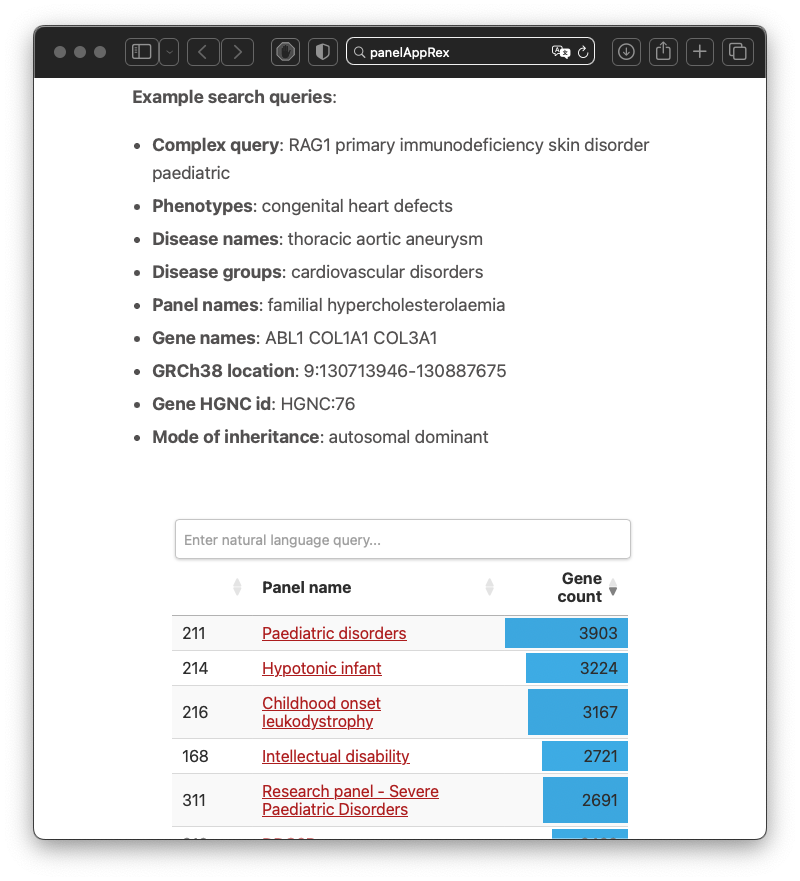
\includegraphics[width=0.49\textwidth]{screenshot_1.png}
    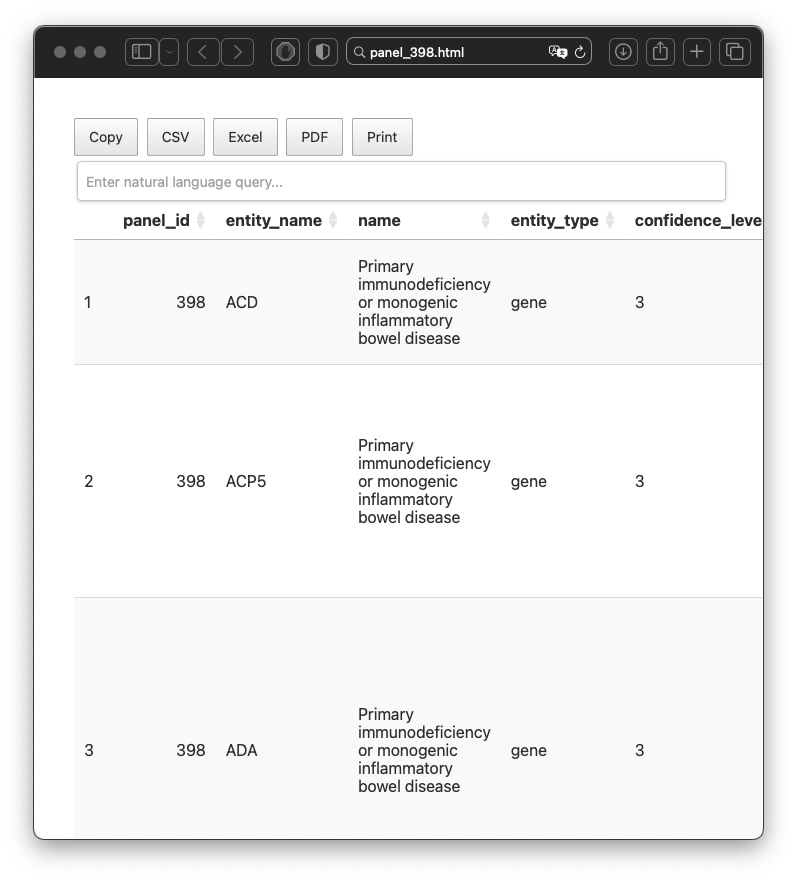
\includegraphics[width=0.49\textwidth]{screenshot_2.png}    
    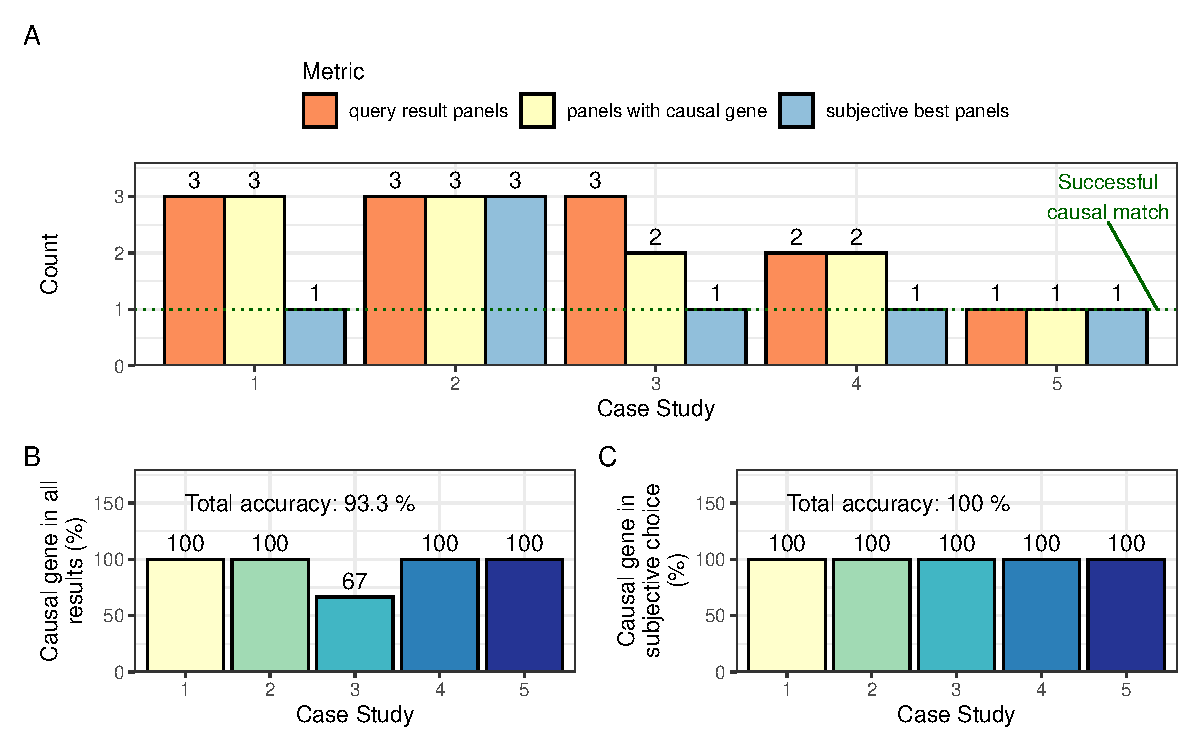
\includegraphics[width=0.85\textwidth]{benchmark.pdf}    
\caption{\textbf{PanelAppRex interface displaying search results for a complex query.} Top: screenshots showing the search interface, with the left panel displaying the full database before filtering and the right panel showing detailed results for a selected panel. Bottom: benchmark metrics are presented as follows: (A) for each of the 5 case studies, the total number of panels returned, the number of panels that included the causal gene, and the single best panel selected (always 1 by default); (B) the percentage of all returned panels that included the true causal gene; (C) the percentage of the single best panels that contained the true causal gene.}
    \label{fig:performance}
\end{figure}

% \FloatBarrier
\subsection{Validation shows completeness in the core dataset}
\noindent
The raw dataset exhibited near-complete coverage in most fields after merging the core dataset. 
Specifically, 99.9915\% of gene entries had \ac{hgnc} symbols % (58587/58592)*100
and 99.2315\% had Ensembl gene IDs. % (57844/58292)*100
All entries included at least one publication, a disease panel name, a \ac{moi}, and an \ac{omim} gene ID (100\% each). 
After recovery of missing identifiers, completeness reached 100\% across all these core fields.
This validated dataset ensures that users can confidently build on a consistent foundation, using standardised and stable identifiers to link or enrich the core data with external resources (\textbf{Figure \ref{fig:validation}}).

\begin{figure}[ht]
    \centering
    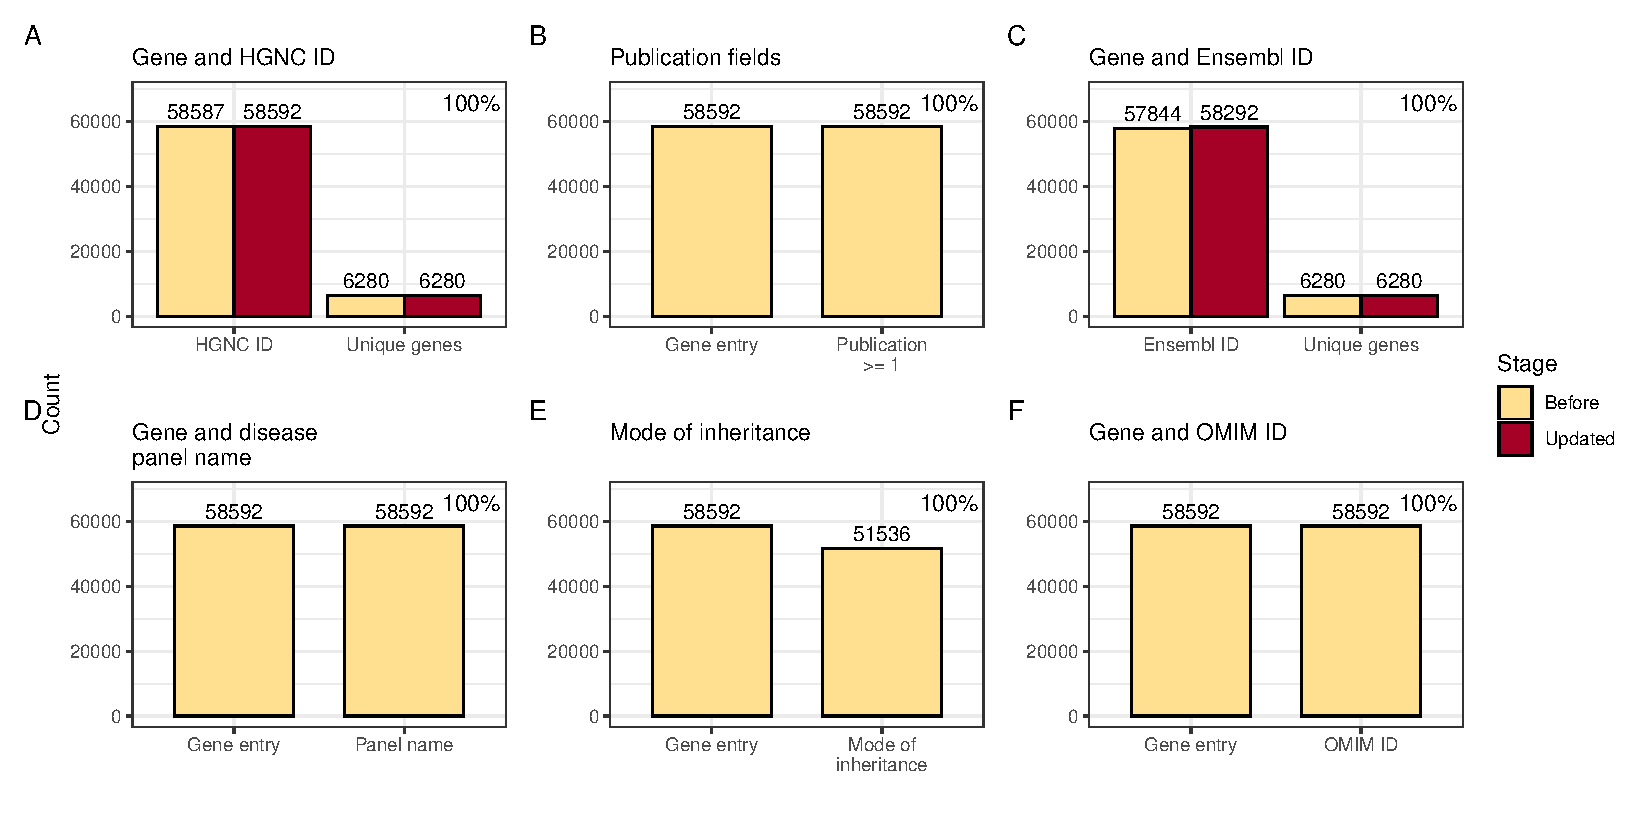
\includegraphics[width=0.99\textwidth]{validation_counts.pdf}
\caption{\textbf{Validation and recovery of core annotation fields in the PanelAppRex dataset.}
(A) Unique genes and HGNC IDs before and after retrieving missing HGNC entries via Ensembl.
(B) Availability of publication annotations for genes.
(C) Unique genes and Ensembl gene IDs before and after biomart-based recovery of missing Ensembl IDs.
(D) Gene entries with associated disease panel names.
(E) Gene entries with annotated \ac{moi}.
(F) Gene entries linked to an OMIM gene ID.
Each bar shows the count of entries with non-missing values for the respective field. Updated fields (HGNC and Ensembl ID) reflect values recovered via external lookup using HGNC symbols. Percentage shows the complete recovery of coverage across features.
}
    \label{fig:validation}
\end{figure}

\subsection{Benchmarking for manual queries confirms accurate retrieval of causal disease genes}
\noindent
To evaluate the practical utility of our system on a desktop browser, we applied the benchmarking approach described in methods using five published case studies of \ac{pid}
\cite{arruda_genetic_2015, 
mcaleer_severe_2015,
verhoeven_hematopoietic_2022,
magerus-chatinet_autoimmune_2013,
sharfe_fatal_2014}. % results
The tool's query process retrieved gene panels using natural language-style input. 
For example, in the first case study on Hereditary Angioedema, the authors reported suspecting that the condition was linked to ``\textit{SERPING1}, Factor XII, and edema" which we used as the query terms. 
Although the true causal gene term \textit{F12} (using its official \ac{hgnc} name) was not mentioned, the inclusion of the alias name and/or related disease terms enabled the system to correctly retrieve the panel containing \textit{F12} based on the hidden search knowledge.

While an expert might readily recognise ``Factor XII'' as an alias name for \textit{F12}, this correct query result demonstrates that the system can make such connections automatically, based on its extensive metadata, supporting users with varying levels of genetic expertise.
Notably, for all five case studies, all correct causal genes were successfully retrieved by the system despite never appearing explicitly in any of our submitted query terms (\textbf{Table \ref{tab:benchmark}}).

In our evaluation, PanelAppRex returned panels in which the causal gene was present in 93\% of all returned panels, with the subjective user-selected ``best panel'' achieving a perfect accuracy of 100\% 
(\textbf{Figure \ref{fig:performance}}).
 These metrics were derived by comparing the causal gene identified from the case study abstracts to the panels returned by our query, and by applying a subjective relevance measure to mimic intuitive panel selection - acknowledging that certain panels, such as the established \ac{pid} gene panel, are inherently more reliable than broader, less specific panels.
 
% (i.e. \ac{pid} panel instead of COVID-19 research panel for  diagnosis of immune disorder}). 
Overall, the results confirm that our approach accurately identifies the most relevant panels and effectively supports clinical decision-making in complex diagnostic scenarios.

\begin{table}[htbp]
\caption{\textbf{Summary of case study queries and PanelAppRex results.} 
``Subjective best panels'' are those reasonably preferable to the clinical query and unlikely to be excluded by users. In the benchmark scenario, broad or less relevant panels (e.g. ``COVID-19 research'') might be deprioritised in favour of more clinically aligned options such as ``Fetal anomalies'', or ``Paediatric disorders''. Summarised in \textbf{Figure \ref{fig:performance}}.
*Case study 5 had five individual cases and patient information was significantly longer than other studies. Therefore, we used OpenAI model o3-mini to converted it to a standardised keyword query automatically, thereby removing our subjective bias and aligning with the other queries.
}
\label{tab:benchmark}
\centering
\resizebox{\textwidth}{!}{
\begin{tabular}{|
    p{1cm}|
    p{4cm}|
    p{4cm}|
    p{1.4cm}|
    p{1.3cm}|
    p{1.3cm}|
    p{1.3cm}|
    p{1.3cm}|
    p{1.3cm}|
    p{5cm}|}
\hline
\textbf{Case study}	(\textbf{Ref})	 & 	\textbf{Source title}	 & 	\textbf{Query}	 & 	\textbf{Causal gene}	 & 	\textbf{Result panels}	 & 	\textbf{Subjective best panels}	 & 	\textbf{Panels with causal gene}	 & 	\textbf{Subjective relevance ratio}	 & 	\textbf{Causal gene in all results}	 & 	\textbf{Result ID, panelName, geneCount} \\
\hline																			
1	\cite{arruda_genetic_2015}	 & 	Genetic Analysis As a Practical Tool to Diagnose Hereditary Angioedema with Normal C1 Inhibitor: A Case Report	 & 	SERPING1 Factor XII edema	 & 	F12	 & 	3	 & 	1	 & 	3	 & 	0.3	 & 	1	 & 	64 COVID-19 research 695; 192 Primary immunodeficiency or monogenic inflammatory bowel disease 572; 311 Research panel - Severe Paediatric Disorders 2691 \\
\hline																			
2	\cite{mcaleer_severe_2015}	 & 	Severe dermatitis, multiple allergies, and metabolic wasting syndrome caused by a novel mutation in the N-terminal plakin domain of desmoplakin	 & 	SAM syndrome DSG1 dermatitis metabolic wasting	 & 	DSP	 & 	3	 & 	3	 & 	3	 & 	1	 & 	1	 & 	205 Fetal anomalies 2185; 210 DDG2P 2422; 211 Paediatric disorders 3903 \\
\hline																			
3	\cite{verhoeven_hematopoietic_2022}	 & 	Hematopoietic stem cell transplantation in a patient with proteasome-associated autoinflammatory syndrome (PRAAS)	 & 	resistant cutaneous vasculitis SH2D1A	 & 	PSMB4	 & 	3	 & 	1	 & 	2	 & 	0.3	 & 	0.7	 & 	64 COVID-19 research 695; 192 Primary immunodeficiency or monogenic inflammatory bowel disease 572; 311 Research panel - Severe Paediatric Disorders 2691 \\
\hline																			
4	\cite{magerus-chatinet_autoimmune_2013}	 & 	Autoimmune lymphoproliferative syndrome caused by a homozygous null FAS ligand (FASLG) mutation	 & 	Autoimmune lymphoproliferative syndrome ALPS lymphoproliferation hypergammaglobulinemia autoimmune cytopenia	 & 	FASLG	 & 	2	 & 	1	 & 	2	 & 	0.5	 & 	1	 & 	64 COVID-19 research 695; 192 Primary immunodeficiency or monogenic inflammatory bowel disease 572 \\
\hline																			
5*	\cite{sharfe_fatal_2014}	 & 	Fatal combined immunodeficiency associated with heterozygous mutation in STAT1	 & 	primary immunodeficiency recurrent pneumonia chronic diarrhea oral thrush bronchiectasis lymphadenopathy hepatosplenomegaly autoimmune hepatitis Addison	 & 	STAT1	 & 	1	 & 	1	 & 	1	 & 	1	 & 	1	 & 	192 Primary immunodeficiency or monogenic inflammatory bowel disease 572 \\
\hline
\end{tabular}
}
\end{table}

\subsection{Structured inheritance annotations reveal overlapping gene-MOI relationships}

To assess the distribution of inheritance annotations we summarised all unique gene-\ac{moi} combinations across 58,592 entries as displayed in 
\textbf{Figure \ref{fig:uniq_gene_moi}}. Among 6,280 distinct genes, a total of 9,237 unique gene-\ac{moi} pairs were identified, reflecting instances where a gene appears with multiple inheritance modes across different panels. 
The most common annotations were \ac{ar} and \ac{ad}, consistent with their prevalence in monogenic disease panels. 
These structured inheritance annotations underpin key applications 
enabled by PanelAppRex, including \ac{moi}-filtered search and model-based prior estimation.


\FloatBarrier
\section{Discussion}
\noindent
PanelAppRex provides an accessible and validated platform for querying, aggregating, and exporting curated disease-gene panel data. Designed for both clinical and research use, it simplifies study planning and variant interpretation through a user-friendly interface, while also offering a harmonised dataset for programmatic workflows. The core model integrates over 58,000 panel-gene associations, with full coverage of key fields including \ac{hgnc} symbols, Ensembl IDs, \ac{omim} annotations, \ac{moi}, and supporting publications.

Beyond immediate usability, PanelAppRex lays a foundation for genome-wide statistical modelling of disease risk. 
With annotations for gene-disease relationships, the dataset provides a core building block towards rigorous estimation of the prior probability of observing  variant classifications (e.g. benign, pathogenic) under different disease \ac{moi}.
%This helps address a persistent challenge in clinical genetics: the lack of principled priors for variant interpretation that account not only for known pathogenic variants (true positives), but also for unobserved variants and negative evidence (false negative causal pathogenic variant and true negative absence of causal variants) \cite{hannah_using_2024, zschocke_mendelian_2023}. 
This addresses a key challenge in clinical genetics: the absence of principled priors for variant interpretation that incorporate not only known pathogenic variants (true positives), but also unobserved pathogenic variants (false negatives) and the absence of pathogenic findings (true negatives) \cite{hannah_using_2024, zschocke_mendelian_2023}.
By integrating high-resolution allele frequencies from gnomAD \cite{karczewski2020mutational}, curated classifications from ClinVar \cite{landrum_clinvar_2018}, and structured gene-disease associations \cite{martin_panelapp_2019}, 
PanelAppRex can enable the derivation of calibrated genome-wide priors for Bayesian models of genetic risk.

These capabilities go beyond panel lookup to support evidence-aware diagnostics. 
Probabilistic models incorporating both observed and unobserved variation can quantify uncertainty, resolve ambiguous findings, and refine variant prioritisation, scaling naturally to support complex, multi-gene disorders. 
The dataset also provides a substrate for AI-driven approaches to variant interpretation, including probabilistic inference, reinforcement learning, and deep annotation pipelines
\cite{jumper_highly_2021, cheng_accurate_2023}.

Several limitations should be acknowledged. Not all known coding genes are currently linked to a disease panel; we prioritised high-confidence, traceable annotations over broad but less reliable coverage. 
Some genes are over-represented across multiple panels due to historical research biases, leading to non-uniform panel enrichment. 
Additionally, not all panels returned by queries may be equally informative. 
For example, during benchmarking, the COVID-19 research panel frequently appeared alongside the \ac{pid} panel due to overlapping genes. 
While technically accurate, such panels may be less relevant to users focused on clinical  diagnosis of immunodeficiency.
% To consider typical user expectations, we included a subjective ``best match'' choice in each case study.
In bioinformatic workflows, these choices can be refined systematically or excluded using filters or downstream logic.
In one of the five case studies, a disease-based query returned three panels, one of which did not contain the causal gene. This is expected, as broader classifications may include non-specific panels, hindering sensitivity. However, the query was still considered 100\% successful, as the causal gene appeared in the combined result set, consistent with the recommended bioinformatic strategy of using the union of returned panels.

PanelAppRex bridges expert-curated panel knowledge with genome-scale statistical reasoning. 
It offers a robust tool for interactive search, a validated dataset for programmatic access, and a scalable framework for quantitative genomic modelling. 
Future work will focus on expanding supported queries, integrating additional variant types and annotations, and enabling more sophisticated applications in variant interpretation and risk estimation.

\section{Conclusion}
\noindent
PanelAppRex offers a robust solution for bioinformatically aggregating and querying gene panel data. Its additional user interface with sophisticated search feature simplifies data exploration and enhances variant interpretation. 

\section*{Acknowledgements}
\noindent
We acknowledge \ac{ge} for providing public access to the PanelApp data.
The use of data from \ac{ge} panelapp was used under the Apache License 2.0.
The use of data from UniProt was licensed under Creative Commons Attribution 4.0 International (CC BY 4.0).
ClinVar asks its users who distribute or copy data to provide attribution to them as a data source in publications and websites \cite{landrum_clinvar_2018}.
Ensembl data and code are available without restriction; software is provided under the Apache License 2.0 \cite{dyer_ensembl_2025}.

\section*{Contributions}
\noindent 
DL designed and performed analyses and wrote the manuscript.
SB, AS, SS, JF, LJS designed analysis and wrote the manuscript.
%JF, LJS supervised the work, and applied for funding.
The Quant Group is a collaboration across multiple institutions where authors contribute equally; the members on this project were DL, SB, and AS.

\section*{Competing interest}
\noindent
The authors declare no competing interest. 

\section*{Ethics statement}
\noindent
This study only used data which was previously published and publicly available, as cited in the manuscript.
This  SwissPedHealth study, under which this work was carried out, was approved based on the advice of the ethical committee Northwest and Central Switzerland (EKNZ, AO\_2022-00018). 
The study was conducted in accordance with the Declaration of Helsinki.

\section*{Funding}
\noindent This project was supported through the grant Swiss National Science Foundation  (SNF) 320030\_201060, and NDS-2021-911 (SwissPedHealth) from the Swiss Personalized Health Network and the Strategic Focal Area `Personalized Health and Related Technologies' of the ETH Domain (Swiss Federal Institutes of Technology).

\section*{Data availability}
\begin{itemize}
\item Data: Lawless, D. (2025). PanelAppRex base Zenodo. \url{https://doi.org/10.5281/zenodo.15736689}
\item Source code: \url{https://github.com/DylanLawless/PanelAppRex}
\item Demonstration page: \url{http://DylanLawless.github.io/panelapprex.github.io/landing_page.html}. 
\end{itemize}

\bibliographystyle{unsrtnat}
\bibliography{references.bib}
\clearpage

%\\\\\\\\\\\\\\\\\\\\\\\\\\\\
\beginsupplement
\section{Supplemental} \label{Supplemental_text}

\begin{figure}[ht]
    \centering
    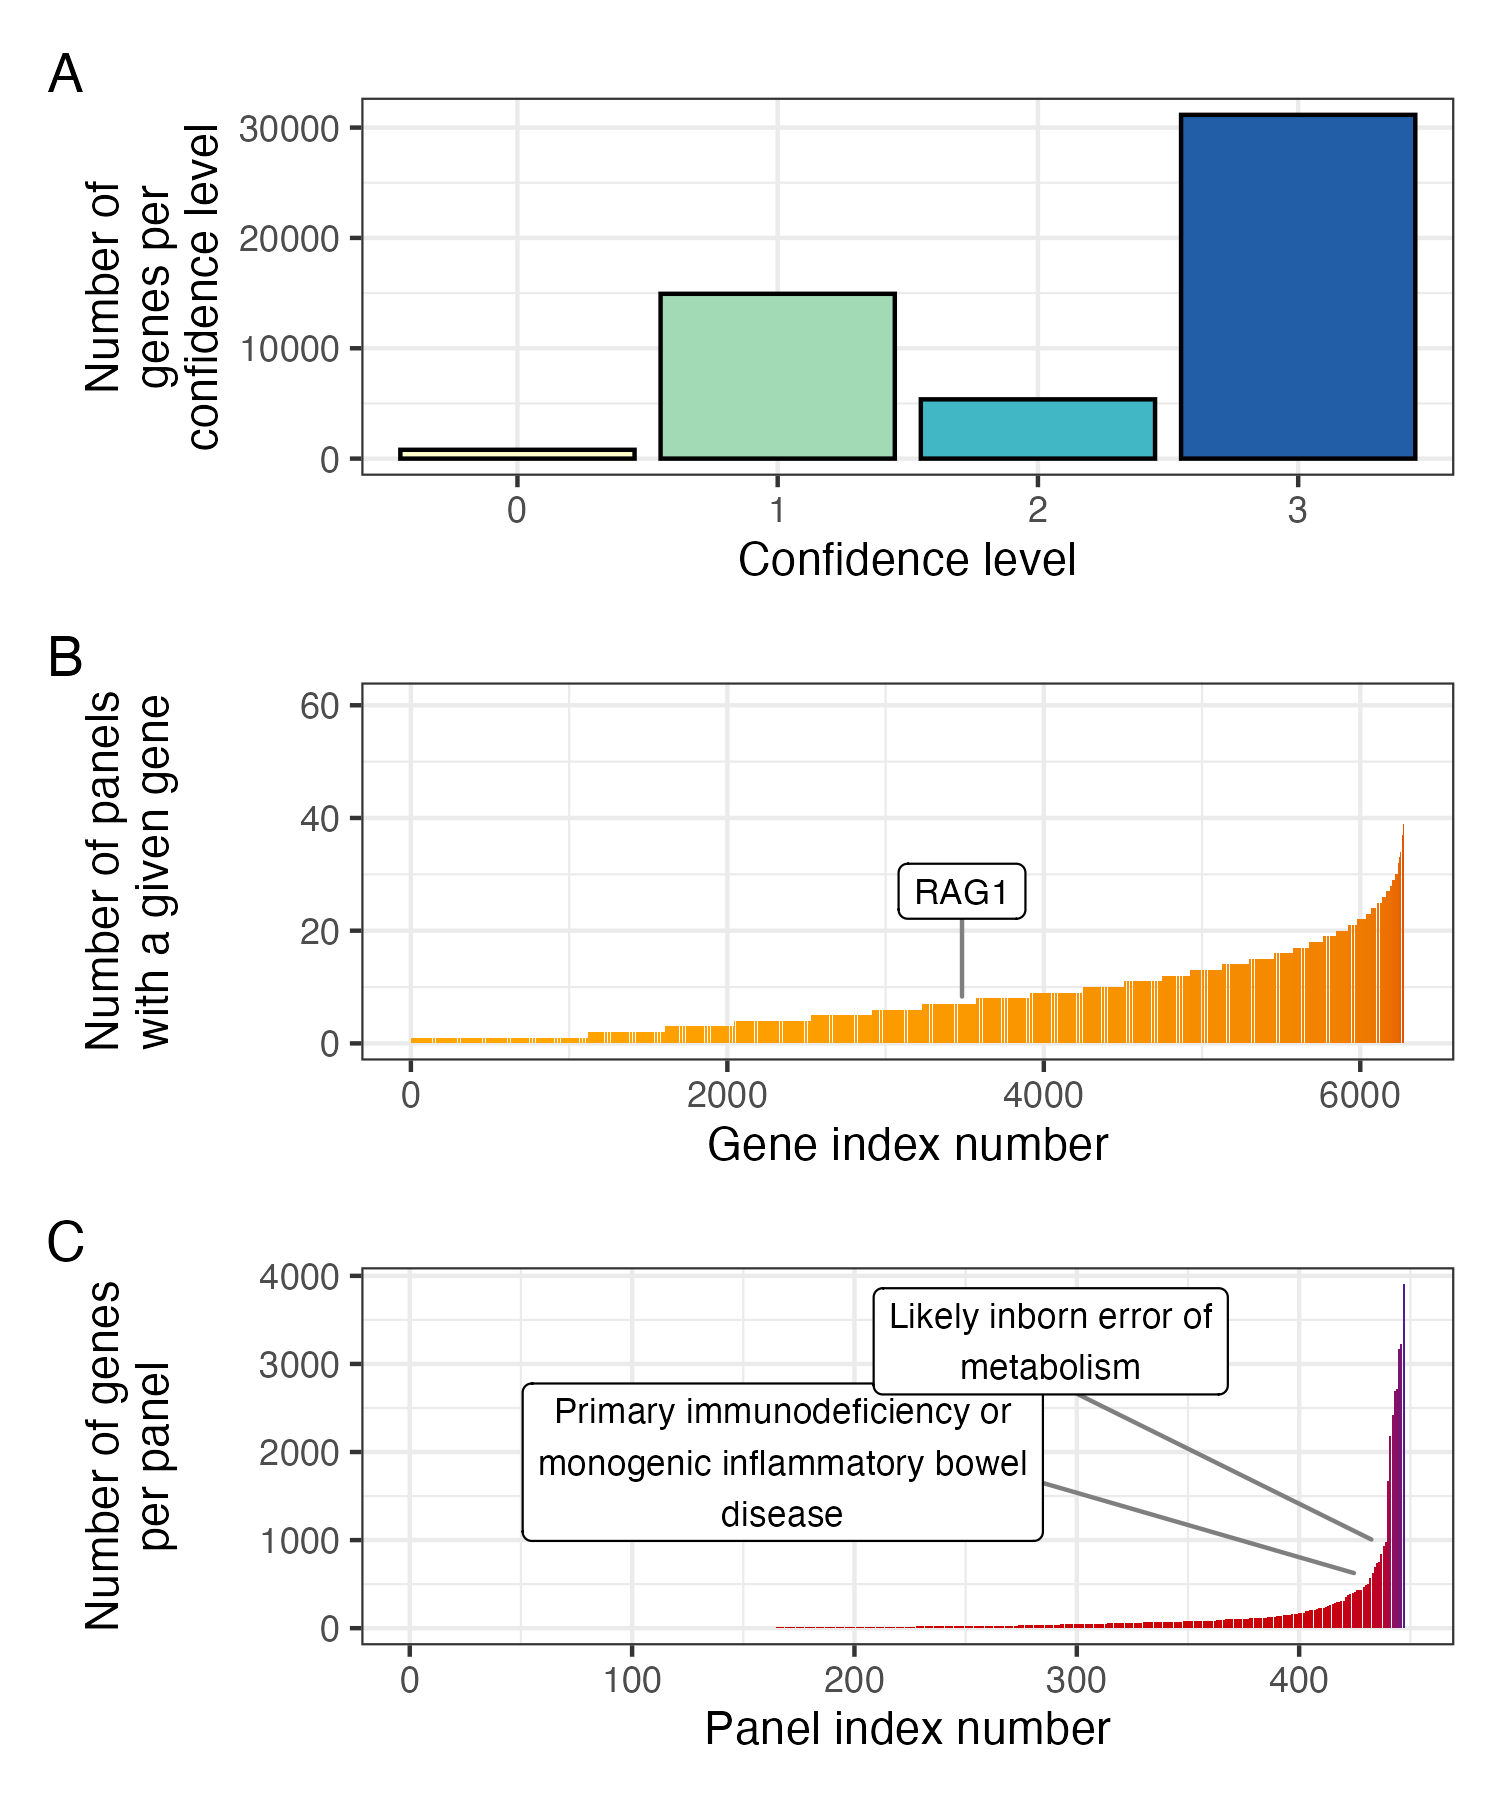
\includegraphics[width=0.75\textwidth]{plot_patch2_annotated_example.png}    
\caption{\textbf{Summary of gene confidence levels, reuse across panels, and panel sizes in the PanelAppRex dataset.}
(A) Number of genes per confidence level. 
(B) Number of panels in which each gene is included, with the example gene \textit{RAG1} highlighted to demonstrate that it is present in 7 panels. 
(C) Number of genes per panel, with two representative panels annotated: panel ID 398 (\ac{pid}/\ac{iei}) and panel ID 1220 (\ac{iem}).
}
    \label{fig:summary_stats}
\end{figure}


\begin{figure}[ht]
    \centering
    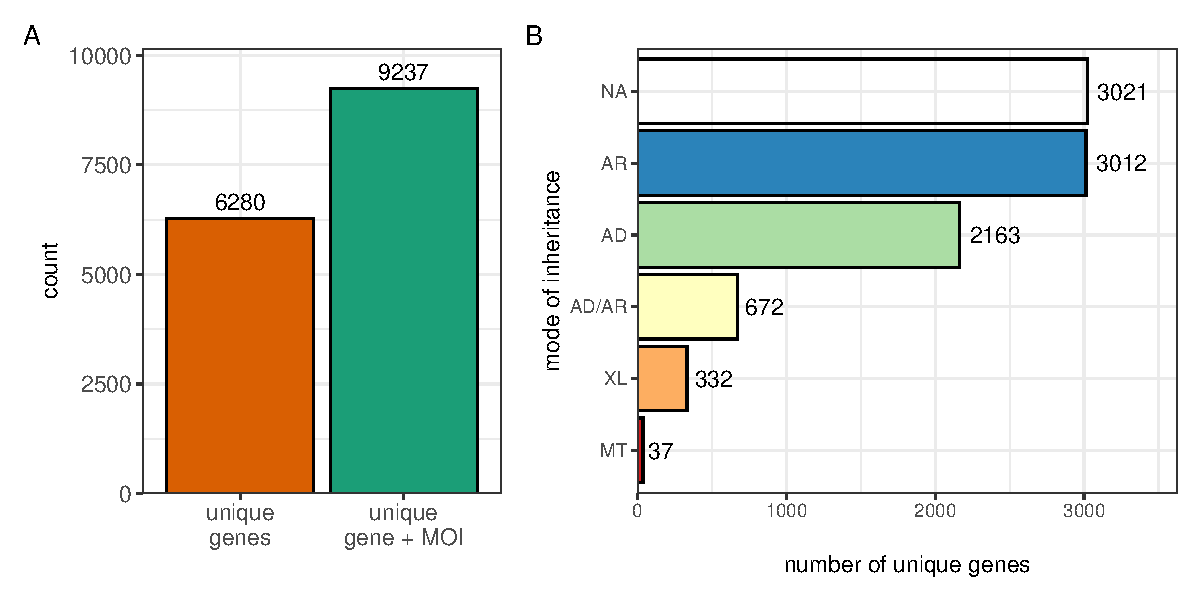
\includegraphics[width=0.99\textwidth]{plot_patch_uniq_gene_moi_summary.pdf}
\caption{\textbf{Summary of mode of inheritance annotations in the PanelAppRex dataset.}
(A) Counts of unique genes annotated with each \ac{moi}, based on non-redundant gene-\ac{moi} combinations.
(B) Total number of unique genes and total number of gene-\ac{moi} combinations in the harmonised PanelAppRex dataset.
}
    \label{fig:uniq_gene_moi}
\end{figure}

\begin{figure}[ht]
    \centering
    
\includegraphics[width=0.99\textwidth]{panelapprex_logo_v2_16x9.png}
\caption{\textbf{(logo)} PanelAppRex reigns over genomic complexity.
}
    \label{fig:uniq_gene_moi}
\end{figure}

\end{document}
